\documentclass{article}
\usepackage[utf8]{inputenc}
\usepackage[spanish]{babel}
\usepackage{listings}
\usepackage{graphicx}
\graphicspath{ {Images/} }
\usepackage{cite}

\begin{document}

\begin{titlepage}
    \begin{center}
        \vspace*{1cm}
            
        \Huge
        \textbf{Informe Escrito}
            
        \vspace{0.5cm}
        \LARGE
        Parcial 2 - Primera parte
            
        \vspace{1.5cm}
            
        \textbf{Julian Taborda Ramirez}
        
        \vspace{0.5cm}
        
        \textbf{Samuel Ruiz Vargas}
            
        \vfill
            
        \vspace{0.8cm}
            
        \Large
        Informatica II\\
        Universidad de Antioquia\\
        Medellín\\
        Septiembre de 2021
            
    \end{center}
\end{titlepage}

\tableofcontents
\vspace*{1.2cm}

\newpage

\section{Analisís del problema}
\label{analisis}

    \begin{flushleft}
    \subsection{Objetivo(s)}
    Nuestro objetivo es simple, necesitamos ser capaces de representar una imagen en una matriz de leds de un tamaño por determinar, de la forma más fiel posible e independiente de la resolución de la imagen, haciendo uso de las técnicas de submuestreo y sobremuestreo. 
    \end{flushleft}
    
    \vspace*{0.5cm}
    
    \begin{flushleft}
    \subsection{Herramientas}
    Como herramientas de hardware tenemos las tiras neopixel, la tarjeta Arduino uno R3. Además probamos las funciones que nos proporicionaron para analizar una imagen. 
    \end{flushleft}
    \vspace*{0.5cm}
    \begin{flushleft}
    \subsection{Problematica(s)}
     Una de las problematicas a la que nos enfrentamos es la forma en la que vamos a tratar la información extraida de la imagen en QT y posteriormente utilizar esa información en tinkercad.
     
     \vspace*{0.1cm}
     
     Otra de las problematicas que tenemos es como redimensionar la imagen, de tal manera que, se adapte a la matriz independientemente a su relación de aspecto.   
    \end{flushleft}
    \vspace*{2cm}

\newpage
    
\section{Esquema de desarrollo algoritmico}
\label{esquema}
    \begin{flushleft}
        
    \subsection{QT}
    El código de QT debe tener la capacidad de recibir una imagen y ser capaz de entregarnos la información necesaria para el desarrollo de la totalidad de nuestro algoritmo; Esta es nuestra prioridad en la etapa mas temprana de nuestro desarrollo y sobre la que se debe basar nuestro proceso.
    \end{flushleft}

    \begin{flushleft}
    Una vez conseguida la primera parte del algoritmo tenemos que proceder a analizar de que forma vamos a tratar la información sustraída de dicha imagen, con el fin de facilitar la lectura una vez en Tinkercad, dicho esto el manejo de tipos de datos será esencial para el correcto desempeño del programa.
    \end{flushleft}
    \vspace*{0.5cm}
    
    
    \subsection{Tinkercad}
    \begin{flushleft}
        Para el desarrollo del código en Tinkercad, pensamos en el flujo de la información de tal manera que podamos recibir la información de QT(La cual esta previamente procesada para no causar conflictos con Tinkercad) y procesarla según dicte el algoritmo que implementemos para realizar la representación de la matriz de Neopixel. 
    \end{flushleft}
        
\newpage
    
\section{Algoritmo implementado}
\label{implementado}
    \begin{flushleft}
        
    \subsection{QT}
    Para el algoritmo implementado en QT,  pensamos en hacer uso de las librerias estandar, para leer y escribir una imagen de tal manera que la información obtenida pueda ser manipulada . De esta manera primero validamos la existencia de la imagen, pidiendo la dirección de esta, luego se procede a cargar con la función ImageRead() y escribimos sus datos con ImageWrite(), finalmente guardamos la información en un  archivo de texto que posteriormente será utilizado para tratar la información en Tinkercad.  
    \end{flushleft}
    
    \vspace{0.5cm}
            
    \begin{figure}[h]
    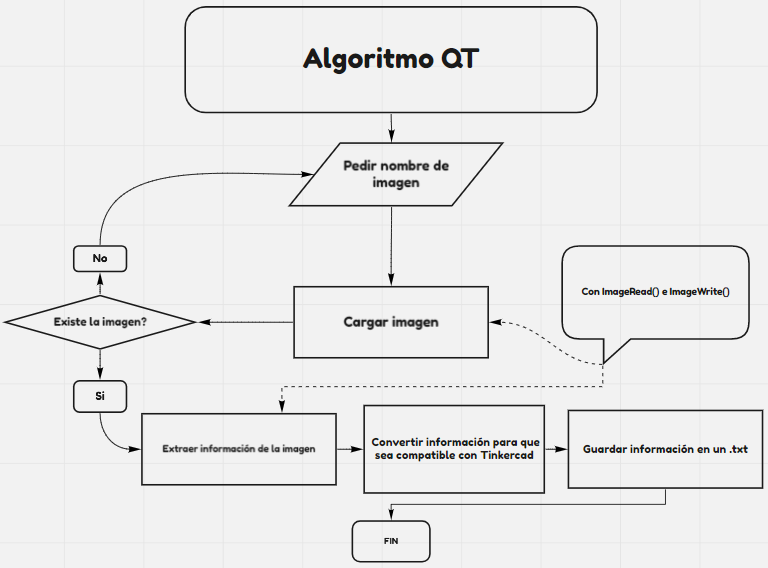
\includegraphics[width=12cm]{Imagenes/diagrama_qt.png}
    \centering
    \label{fig:ram}
    \end{figure}
    \vspace{0.5cm}

    \newpage
    
    \subsection{Tinkercad}
    \begin{flushleft}
    En Tinkercad tomaremos la información correspondiente de la imagen guardada en una archivo de texto, esta se pide haciendo uso de un buffer, aplicando alguna técnica de muestreo (Submuestreo o Sobremuestreo) podremos escalar la imagen de tal manera que se adecue a la cantidad leds que tenemos en la matriz; Claramente debemos tener en cuenta el escalamiento correspondiente ya que debemos mantener una fidelidad con la relación aspecto de la imagen. Finalmente los leds deben estar encendidos hasta que el programa finalice.
    
    \end{flushleft}
    
    \vspace{0.2cm}
            
    \begin{figure}[h]
    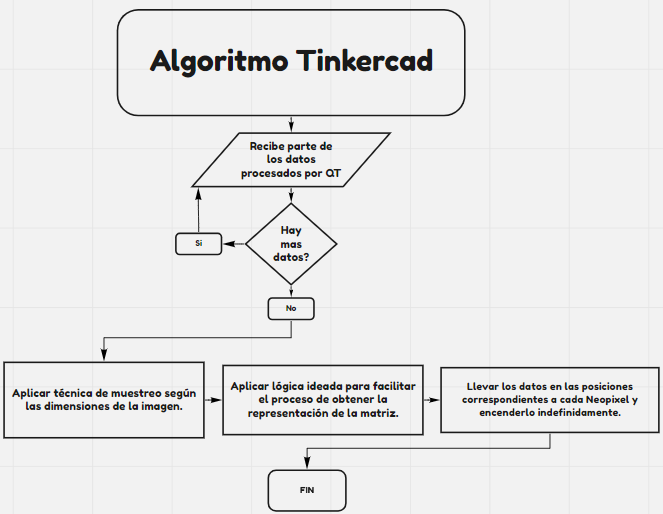
\includegraphics[width=12cm]{Imagenes/diagrama_tinker.png}
    \centering
    \label{fig:ram}
    \end{figure}
    \vspace{0.3cm}
    
\section{Consideraciones}
\label{consideraciones}
    \begin{flushleft}
        Debemos de tener en cuenta la cantidad de leds que tenemos en la matriz ya que, dependiendo de la cantidad de pixeles de la imagen se tiene que aplicar cualquiera de la dos tecnicas, para adaptar la imagen a la cantidad de leds de la matriz.
        
        \vspace*{0.1cm}
        
        A su vez debemos determinamos algunas cosideracciones lógicas para el tratamiento de la imagen, en este caso los colores dominantes y algunas configuraciones geometricas para representar la imagen.
    \end{flushleft}
    

\vfill
\bibliographystyle{IEEEtran}


\end{document}